\subsection{OriginStamp i Blockchain}
\label{arquitectura:blockchain}
%With the advent of cryptocurrencies like Bitcoin, it has become possible to securely timestamp information in a decentralized and tamper-proof manner. Digital data can be hashed and the hash can be incorporated into a transaction stored in the blockchain, which serves as a secure proof of the exact time at which that data existed[2]. The proof is due to a tremendous amount of computational effort performed after the hash was submitted to the blockchain. Tampering with the timestamp would also lead to breaking the integrity of the entire digital currency, and this would result in the digital currency devaluing to zero[3].
%The decentralized timestamping approach using the Blockchain has also found applications in other areas, such as in dashboard cameras, to secure the integrity of video files at the time of their recording,[4] or to prove priority for creative content and ideas shared on social media platforms
Amb l'avanç de les anomenades criptomonedes (\textit{criptocurrencies} en anglès) com \textit{Bitcoin}, esdevé possible la creació de segells de temps d'una forma segura, descentralitzada i no modificable.\\
%\newline Així doncs, el \textit{hash} dels documents es poden incorporar a les transaccions i aquestes ser emmagatzemades a la \textit{blockchain}, que serveix com a prova de que en un instant determinat la informació a partir de la qual s'ha generat el \textit{hash}, existia.\\
%\newline El caràcter distribuït de la \textit{blockchain}, otorga irrefutabilitat a la prova d'existència, ja que ràpidament quedarà replicada als diferents nodes, aconseguint que la modificaició d'aquesta, sigui computacionalemnt impossible.\\
%\newline Així doncs serveis com \textit{OriginStamp}\footnote{https://app.originstamp.org/home} ofereixen la possibilitat de fer servir \textit{blockchain} per a certificar informació, en el context del TFG, el contingut dels comprovants de signatura generats.
%\begin{figure}[h]
%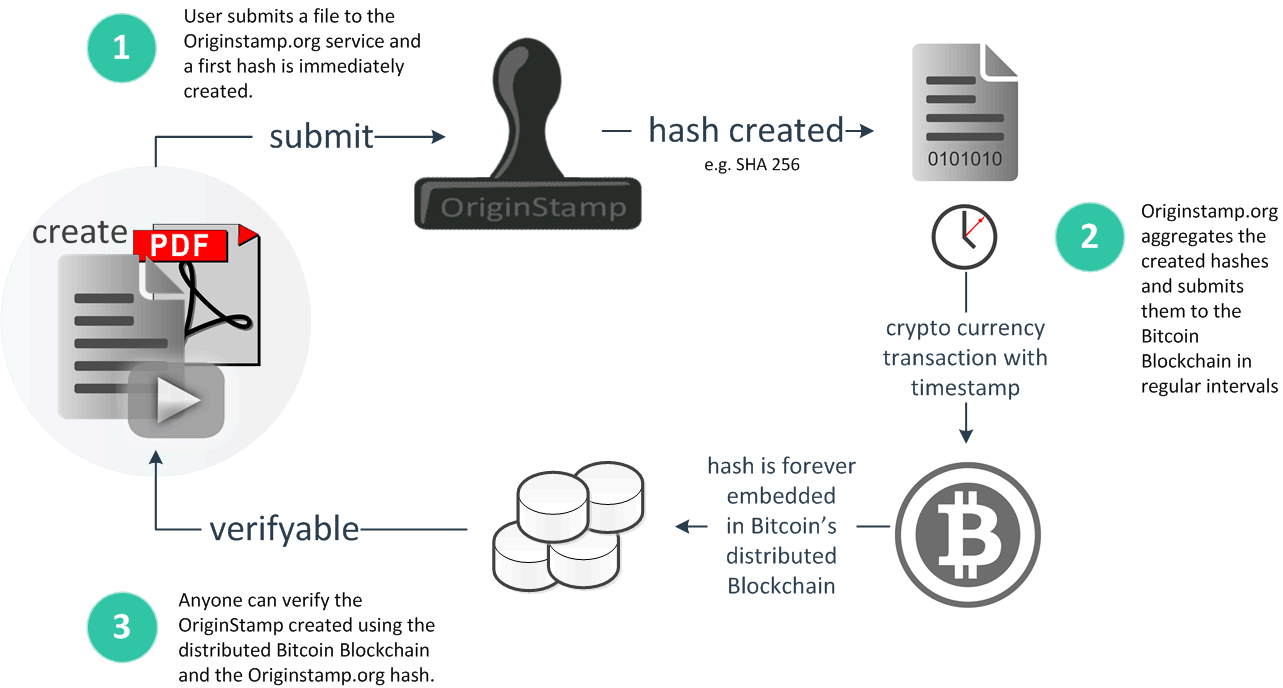
\includegraphics[scale=0.6]{sections/arquitectura/originStamp_workflow.png}
%\centering
%\caption{Funcionament d'OriginStamp}
%\label{fig:originstamp_workflow}
%\end{figure}
%\newline La Figura \ref{fig:originstamp_workflow} mostra el funcionament del servei \textit{OriginStamp}.\\
%Després de l'obtenció de la corresponent \textit{APIKey} per a poder realitzar operacions, manca encapsular les diferents funcionalitats en funcions php que facin les corrsponents crides a la API d'\textit{OriginStamp}.
\newline En el cas d'aquest TFG la creació d'un segell de temps és indispensable per a poder assolir l'objectiu final satisfactòriament.\\
\newline Al llarg d'aquesta secció es donaran detalls sobre els segon dels casos d'ús que es mostren a la Figura \ref{fig:hash_timestamping_usecase}, en concret al cas d'ús ``publicar hash a la blockchain''.\\
\newline De la mateixa manera que el component descrit a la secció \ref{arquitectura:generacio_documents}, aquest cas d'ús es composa de dos parts:
\begin{itemize}
    \item Un dels serveis del \textit{backend} desenvolupat, específicament per encapsular aquest cas d'ús i poder-lo fer servir des de qualsevol punt del projecte.
    Aquest servei respón a la necessitat d'un adaptador per a que el \textit{backend} es pugui comunicar amb el servei extern
    \item I per l'altre, el servei extern que permet publicar el \textit{hash} a la blockchain de bitcoin.\\
    Aquest servei extern, està dissenyat com una API Rest
\end{itemize}
La comunicació entre ambdós components es realitza a través de crides \textit{HTTP/Get} i \textit{HTTP/Post}, definides a documentació del servei.

